\subsection{Caça Níquel}
% p01q03 prova 2016_1
% ~/ee/ufsj/2016_01/ti/prova/prova01-resolucao.tex

\begin{questions}
\question{
Diante da crise econômica, o Palácio do Planalto está elaborando uma pesquisa ampla
para ``avaliar os impactos da eventual liberação de cassinos no Brasil e os
possíveis modelos de exploração de jogos de azar''
\footnote{\url{http://g1.globo.com/politica/noticia/2016/01/governo-faz-estudo-sobre-impacto-da-liberacao-de-cassino-e-bingo-no-brasil.html}}.
Você foi escolhido para planejar a máquina caça níquel tupiniquim.
Esta máquina deverá funcionar da seguinte maneira:
para jogar, você precisa inserir uma moeda de R\$1,00 e poderá ter 3 (três)
resultados distintos: 
\begin{inparaenum}[1)]
\item perder (não recebe de volta o R\$1,00 depositado),
        ou seja, sai no prejuízo de R\$1,00; 
\item ganhar R\$1,00 (apenas recebe de volta
        o que foi depositado), não sai no prejuízo, nem no lucro;
\item ganhar R\$5,00 (recebe o R\$1,00 depositado acrescido de uma bonificação de R\$4,00),
        sai com um lucro de R\$4,00.
\end{inparaenum}
Esta máquina deverá ser projetada atendendo ainda
a dois requisitos: 
\begin{inparaenum}[a)]
\item o lucro esperado do jogador deverá ser nulo (R\$0,00);
\item os resultados produzidos pela máquina deverão apresentar incerteza máxima,
ou seja, a maior aleatoriedade possível.
\end{inparaenum}
Vamos chamar de $p = (p_1, p_2, p_3)$ a distribuição de massa sobre os possíveis
resultados (1), (2) e (3), conforme acima descritos.
Determine como devemos proceder para encontrar essa distribuição de massa
de forma a satisfazer também os requisitos (a) e (b).
Escreva as equações e relações pertinentes e proponha uma forma (algorítmica e algébrica)
para encontrar esta distribuição de massa.
Encontre algebricamente a distribuição de massa desejada.
}

\begin{solution}
  Devemos encontrar a distribuição que maximiza a entropia, sujeito ao valor esperado do lucro ser nulo.
  Vamos definir a v.a. $X$ com sendo o lucro. Teremos então
  $p_1 = P(X = -1)$, $p_2 = P(X = 0)$ e $p_3 = P(X = 4)$.


  Queremos que o lucro esperado seja nulo,
  \begin{equation}
  E [X] = p_1 \times (-1) + p_2 \times 0 + p_3 \times 4 = 0 .
  \end{equation}
  Assim podemos concluir que $p_1 = 4 p_3$.
  Além disso, temos que $p_1 + p_2 + p_3 = 1$, logo teremos $p_2 = 1 - 5p_3$.
  Podemos escrever então
  \begin{eqnarray}
  H(p) &=& H(p_1, p_2, p_3) \\
       &=& H(4p_3, 1-5p_3, p_3) \\
       &=& - 4p_3 \log 4p_3 - (1-5p_3) \log (1-5p_3) - p_3 \log p_3 .
  \end{eqnarray}
  Note que, devemos ter $p_i \in [0, 1]$, $i=1,2,3$. Podemos assim concluir
  que $p_3 \in [0, 0.2]$ para que os demais $p_i$ também estejam no intervalo $[0, 1]$.

  Sabemos que $H(p)$ é uma função concava em $p$.
  %(no formulário temos $D(p||u)$ é convexo e $H(p) = \log \vert \mathcal{X} \vert - D(p||u)$).
  Isto implica a existência de um ponto de máximo absoluto.
  Podemos encontrar este ponto de máximo através de um algoritmo de maximização
  (como o método do gradiente) ou algebricamente.

  Para determinar algebricamente, devemos encontrar o valor de $p_3$ que faça
  $\partial H / \partial p_3 = 0$,
  \begin{eqnarray}
  \frac{\partial H}{\partial p_3} &=& - 4 \log 4p_3 - 4p_3 \frac{1}{4p_3} 4 - (-5) \log (1-5p_3) - (1-5p_3) \frac{1}{(1-5p_3)}(-5) - \log p_3 - p_3 \frac{1}{p_3} - 1 \\
          &=& - 4 \log 4p_3 + 5 \log (1-5p_3) - \log p_3 = 0
  \end{eqnarray}

  ou seja, devemos ter
  \begin{eqnarray}
  \log \frac{(1-5p_3)^5}{ (4p_3)^4 p_3 } &=& 0 \\
  \log \frac{(1-5p_3)^5}{ 4^4 p_3^5 } &=& 0 \\
  \frac{(1-5p_3)^5}{ 4^4 p_3^5 } &=& 1 \\
  \frac{1-5p_3}{4^{4/5} p_3} &=& 1 \\
  1-5p_3 &=& 2^{8/5} p_3 \\
  p_3 &=& \frac{1}{5 + 2^{8/5}} \approx 0.12451 .
  \end{eqnarray}
  Podemos agora determinar $p_1$ e $p_2$ utilizando as relações vistas anteriormente.
  Teremos assim
  \noindent\begin{minipage}{.33\linewidth}
  \begin{equation}
    p_1 = \frac{4}{5 + 2^{8/5}}
  \end{equation}
  \end{minipage}%
  \begin{minipage}{.33\linewidth}
  \begin{equation}
    p_2 = \frac{2^{8/5}}{5 + 2^{8/5}}
  \end{equation}
  \end{minipage}%
  \begin{minipage}{.33\linewidth}
  \begin{equation}
    p_3 = \frac{1}{5 + 2^{8/5}}
  \end{equation}
  \end{minipage}

  Abaixo é apresentado um código onde é utilizado o método do gradiente 
  para encontrar numericamente a solução.

\begin{lstlisting}[language=Octave]
p = [0.01 : 0.01 : 0.19];
H = - 4*p.*log2(4*p) - (1-5*p).*log2(1- 5*p) - p.*log2(p);
figure; plot(p,H);
xlabel('p3'); ylabel('H');

% metodo gradiente
alfa = 0.01; eps = 1E-3;
p3 = 0.1;
for i=1:1E3, 
    dH = -4*log2(4*p3) + 5*log2(1-5*p3) - log2(p3); 
    p3 = p3 + alfa * dH; 
    if abs(dH) < eps, break; end; 
end;

H3 = - 4*p3.*log2(4*p3) - (1-5*p3).*log2(1- 5*p3) - p3.*log2(p3);
line([0 p3], [H3 H3], 'LineStyle','--');
line([p3 p3], [0.2 H3], 'LineStyle','--');

set(gca, 'Box', 'off');
print -dsvg niquel.svg;
system('inkscape niquel.svg --export-pdf=niquel.pdf');
% comparacao com o resultado analitico
p3 - 1 / (2^(8/5) + 5)
\end{lstlisting}

  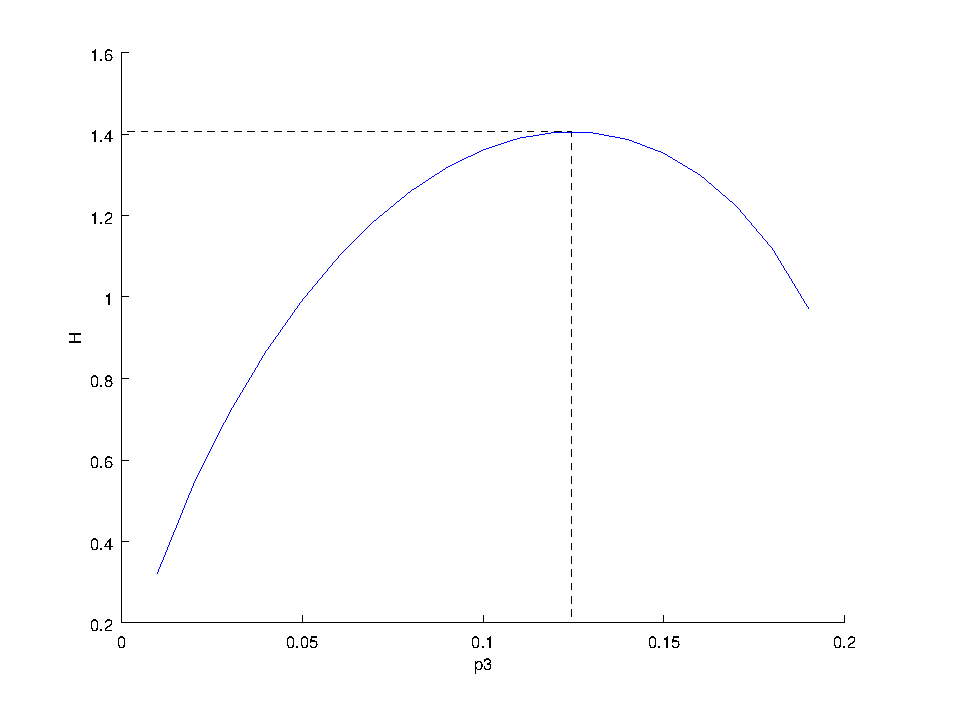
\includegraphics[width=0.5\textwidth]{../images/niquel.pdf}


\end{solution}
\end{questions}
